\documentclass[border=2pt]{standalone}
\usepackage{tikz}
\usetikzlibrary{arrows.meta,positioning,calc,fit,backgrounds,shapes.geometric}
\usepackage{amsmath,amssymb}
\usepackage{times}
\definecolor{ink}{HTML}{243447}
\definecolor{cA}{HTML}{4477AA}
\definecolor{cB}{HTML}{CC6677}
\definecolor{cAu}{HTML}{44AA99}
\definecolor{cS}{HTML}{CCAA33}
\definecolor{grn}{HTML}{228833}
\definecolor{rose}{HTML}{AA3377}
\definecolor{inst}{HTML}{F2E3B3}
\tikzset{
 pap/.style={circle,draw=ink,line width=.6pt,minimum size=15pt,inner sep=0pt,font=\scriptsize\bfseries,text=white},
 aut/.style={rectangle,draw=ink,line width=.6pt,minimum size=13pt,inner sep=0pt,fill=cAu,font=\scriptsize\bfseries,text=white},
 sub/.style={diamond,draw=ink,line width=.6pt,minimum size=17pt,inner sep=0pt,fill=cS,font=\scriptsize\bfseries,text=white},
 gone/.style={draw=ink!35,fill=ink!8,text=ink!40,dashed},
 ed/.style={draw=ink,line width=.7pt},
 msg/.style={-{Stealth[length=4pt]},line width=.9pt,draw=rose},
 ptitle/.style={font=\footnotesize\bfseries,text=ink,anchor=west},
 note/.style={font=\scriptsize,text=ink,align=center},
}

\tikzset{
 est/.style={rectangle,draw=grn,fill=grn!15,line width=.6pt,minimum size=7pt,inner sep=0pt},
 fst/.style={circle,fill=rose,inner sep=2.2pt},
 stage/.style={draw=ink!50,rounded corners=3pt,line width=.6pt,minimum height=4.75cm,anchor=north west,fill=white},
 stnum/.style={circle,fill=ink,text=white,font=\scriptsize\bfseries,inner sep=1.4pt},
 sname/.style={font=\footnotesize\bfseries,text=ink,anchor=west},
 txt/.style={font=\scriptsize,text=ink,align=center},
 vec/.style={draw=ink,fill=#1,minimum width=3.6pt,minimum height=8pt,inner sep=0pt},
 flow/.style={-{Stealth[length=5pt]},line width=1.2pt,draw=ink!60},
 mp/.style={-{Stealth[length=3.5pt]},grn,line width=.9pt},
 nf/.style={rose,line width=.55pt},
 ef/.style={grn!80!black,line width=.75pt},
 grad/.style={-{Stealth[length=4pt]},line width=.8pt,draw=cB!85!black,dashed},
}
\newcommand{\vbars}[3]{\foreach \k in {1,2,3}{\node[vec=#3] at ($(#1)+(#2)+(\k*0.13,0)$) {};}}
\begin{document}
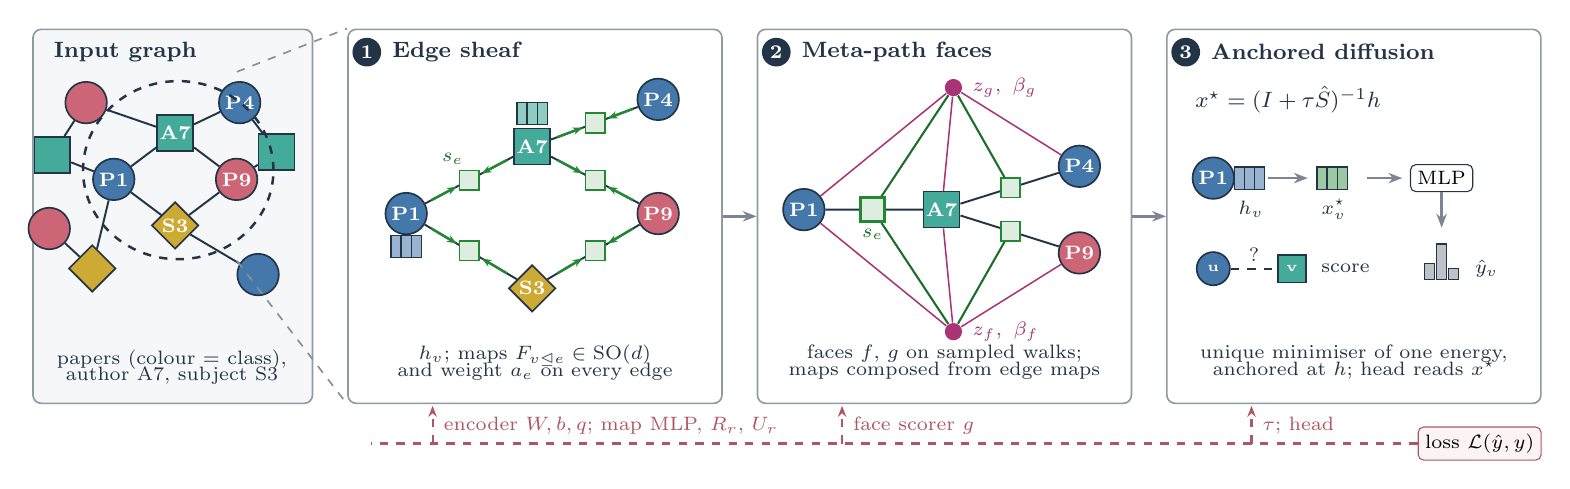
\begin{tikzpicture}
\def\WI{3.55}\def\WP{4.75}\def\G{0.45}
\pgfmathsetmacro{\xA}{\WI+\G}
\pgfmathsetmacro{\xB}{\xA+\WP+\G}
\pgfmathsetmacro{\xC}{\xB+\WP+\G}
\node[stage,minimum width=\WI cm,fill=ink!4] (BI) at (0,0) {};
\node[sname] at (0.15,-0.3) {Input graph};
\foreach \i/\x/\t in {1/\xA/Edge sheaf,2/\xB/Meta-path faces,3/\xC/Anchored diffusion}{
  \node[stage,minimum width=\WP cm] (B\i) at (\x,0) {};
  \node[stnum] at ($(B\i.north west)+(0.25,-0.3)$) {\i};
  \node[sname] at ($(B\i.north west)+(0.45,-0.3)$) {\t};
}
% ---------- input graph
\begin{scope}[shift={(0.1,-0.2)},scale=0.78]
 \node[pap,fill=cA] (iP1) at (1.2,-2.2) {P1};
 \node[aut] (iA7) at (2.2,-1.45) {A7};
 \node[sub] (iS3) at (2.2,-2.95) {S3};
 \node[pap,fill=cB] (iP9) at (3.2,-2.2) {P9};
 \node[pap,fill=cA] (iP4) at (3.25,-0.95) {P4};
 \node[pap,fill=cB] (iP2) at (0.75,-0.95) {};
 \node[aut] (iA2) at (0.2,-1.8) {};
 \node[pap,fill=cA] (iP6) at (3.55,-3.75) {};
 \node[sub] (iS4) at (0.85,-3.65) {};
 \node[pap,fill=cB] (iP7) at (0.15,-3.0) {};
 \node[aut] (iA5) at (3.85,-1.75) {};
 \draw[ed] (iP1)--(iA7) (iA7)--(iP9) (iA7)--(iP4) (iP1)--(iS3) (iS3)--(iP9)
           (iA2)--(iP2) (iA2)--(iP1) (iS3)--(iP6) (iP2)--(iA7) (iS4)--(iP7) (iS4)--(iP1) (iA5)--(iP9) (iA5)--(iP4);
 \draw[ink,dashed,line width=.9pt] (2.25,-2.05) ellipse (1.55 and 1.45);
\end{scope}
\node[txt] at (\WI/2,-4.3) {papers (colour = class),\\[-2pt]author A7, subject S3};
\draw[dashed,ink!55,line width=.6pt] (2.6,-0.55)--(B1.north west);
\draw[dashed,ink!55,line width=.6pt] (2.6,-2.95)--(B1.south west);
% ---------- 1 edge sheaf
\begin{scope}[shift={(\xA+0.75,-2.35)}]
 \node[pap,fill=cA] (aP1) at (0,0) {P1};
 \node[aut] (aA7) at (1.6,0.85) {A7};
 \node[sub] (aS3) at (1.6,-0.95) {S3};
 \node[pap,fill=cB] (aP9) at (3.2,0) {P9};
 \node[pap,fill=cA] (aP4) at (3.2,1.45) {P4};
 \draw[ed] (aP1)--(aA7) (aA7)--(aP9) (aA7)--(aP4) (aP1)--(aS3) (aS3)--(aP9);
 \foreach \u/\v in {aP1/aA7,aA7/aP9,aA7/aP4,aP1/aS3,aS3/aP9}{
   \node[est] at ($(\u)!0.5!(\v)$) {};
   \draw[mp] ($(\u)!0.2!(\v)$)--($(\u)!0.4!(\v)$); \draw[mp] ($(\v)!0.2!(\u)$)--($(\v)!0.4!(\u)$);}
 \node[grn!80!black,font=\scriptsize,anchor=south east] at ($(aP1)!0.5!(aA7)+(0.05,0.08)$) {$s_e$};
 \vbars{aP1}{-0.26,-0.42}{cA!55}
 \vbars{aA7}{-0.26,0.42}{cAu!60}
\end{scope}
\node[txt,anchor=north] at ($(B1.north)+(0,-3.9)$) {$h_v$; maps $F_{v\trianglelefteq e}\in\mathrm{SO}(d)$\\[-2pt]and weight $a_e$ on every edge};
% ---------- 2 meta-path faces
\begin{scope}[shift={(\xB+0.6,-2.3)}]
 \node[pap,fill=cA] (bP1) at (0,0) {P1};
 \node[aut] (bA7) at (1.75,0) {A7};
 \node[pap,fill=cB] (bP9) at (3.5,-0.55) {P9};
 \node[pap,fill=cA] (bP4) at (3.5,0.55) {P4};
 \draw[ed] (bP1)--(bA7) (bA7)--(bP9) (bA7)--(bP4);
 \node[est,minimum size=8.5pt,line width=1.1pt] (be) at ($(bP1)!0.5!(bA7)$) {};
 \node[est] (bf) at ($(bA7)!0.5!(bP9)$) {};
 \node[est] (bg) at ($(bA7)!0.5!(bP4)$) {};
 \node[fst] (zf) at (1.9,-1.55) {};
 \node[fst] (zg) at (1.9,1.55) {};
 \foreach \n in {bP1,bA7,bP9} \draw[nf] (zf)--(\n);
 \foreach \n in {bP1,bA7,bP4} \draw[nf] (zg)--(\n);
 \foreach \e in {be,bf} \draw[ef] (zf)--(\e);
 \foreach \e in {be,bg} \draw[ef] (zg)--(\e);
 \node[rose,font=\scriptsize,anchor=west] at ($(zf)+(0.12,0)$) {$z_f,\ \beta_f$};
 \node[rose,font=\scriptsize,anchor=west] at ($(zg)+(0.12,0)$) {$z_g,\ \beta_g$};
 \node[grn!80!black,font=\scriptsize,anchor=north] at ($(be)+(0,-0.12)$) {$s_e$};
\end{scope}
\node[txt,anchor=north] at ($(B2.north)+(0,-3.9)$) {faces $f$, $g$ on sampled walks;\\[-2pt]maps composed from edge maps};
% ---------- 3 anchored diffusion
\begin{scope}[shift={(\xC+0.25,-0.75)}]
 \node[txt,font=\footnotesize,anchor=west] at (0,-0.15) {$x^\star=(I+\tau\hat S)^{-1}h$};
 \node[pap,fill=cA] (cP1) at (0.35,-1.15) {P1};
 \vbars{cP1}{0.2,0}{cA!55}
 \draw[flow,line width=.9pt] (1.05,-1.15)--(1.55,-1.15);
 \vbars{cP1}{1.25,0}{grn!45}
 \node[txt] at (0.83,-1.55) {$h_v$}; \node[txt] at (1.88,-1.55) {$x^\star_v$};
 \draw[flow,line width=.9pt] (2.3,-1.15)--(2.75,-1.15);
 \node[draw=ink,rounded corners=2pt,fill=white,font=\scriptsize,inner sep=2.5pt] (mlp) at (3.25,-1.15) {MLP};
 \draw[flow,line width=.9pt] (mlp.south)--++(0,-0.45);
 \foreach \k/\h in {1/6,2/13,3/4}{\node[vec=ink!30,minimum height=\h pt,anchor=south] at (2.95+\k*0.15,-2.45) {};}
 \node[txt,anchor=west] at (3.55,-2.3) {$\hat y_v$};
 \node[pap,fill=cA,minimum size=12pt,font=\tiny\bfseries] (lu) at (0.35,-2.3) {u};
 \node[aut,minimum size=10pt,font=\tiny\bfseries] (lv) at (1.35,-2.3) {v};
 \draw[ink,dashed,line width=.7pt] (lu)--(lv) node[midway,above=-1pt,font=\scriptsize]{?};
 \node[txt,anchor=west] at (1.6,-2.3) {score};
\end{scope}
\node[txt,anchor=north] at ($(B3.north)+(0,-3.9)$) {unique minimiser of one energy,\\[-2pt]anchored at $h$; head reads $x^\star$};
% ---------- flows
\draw[flow] (B1.east)--(B2.west);
\draw[flow] (B2.east)--(B3.west);
% ---------- loss and gradients
\pgfmathsetmacro{\yL}{-5.05}
\node[draw=cB!85!black,rounded corners=2pt,fill=cB!8,font=\scriptsize,inner sep=2.5pt,anchor=east] (loss) at ($(B3.south east)+(0,-0.5)$) {loss $\mathcal{L}(\hat y,y)$};
\draw[cB!85!black,dashed,line width=.8pt] (loss.west)--($(B1.south west)+(0.3,-0.5)$);
\foreach \b/\lab in {B1/{encoder $W,b,q$; map MLP, $R_r$, $U_r$},B2/{face scorer $g$},B3/{$\tau$; head}}{
  \draw[grad] ($(\b.south)+(-1.3,-0.5)$)--($(\b.south)+(-1.3,-0.02)$);
  \node[font=\scriptsize,text=cB!85!black,anchor=west,fill=white,inner sep=1pt] at ($(\b.south)+(-1.2,-0.27)$) {\lab};
}
\end{tikzpicture}
\end{document}
